\documentclass[english]{beamer}
\usepackage[english]{babel}
\usepackage{minted}
\usepackage{amsmath}
\usepackage{physics}
\newtheorem*{remark}{Remark}

\usetheme{Rochester}


\title[Finding Maximal Exact Matches in Graph]{Finding Maximal Exact Matches in Graph}
\author{G. Trapani}
\institute{Universit\`a di Pisa}
\date{13/05/2024}
\titlegraphic{\includegraphics[height=1.5cm]{images/unipi-marchio.eps}}
\begin{document}

\frame{\titlepage}
\logo{
	\includegraphics[height=1cm]{images/unipi-marchio.eps}
}
\setbeamercovered{transparent}

\begin{frame}
	\frametitle{Contents}
	\begin{enumerate}
		\item Prerequisites: BWT Transform, Elastic Founder Graph.
		\item Algorithm to find \(\kappa\)-node MEMs.
		\item Algorithm to find \(\kappa\)-node-MEMs spanning exactly \(L\) nodes.
		\item Algorithm to find \(\kappa\)-node-MEMs in EFGs.
		\item Experimental results.
	\end{enumerate}

\end{frame}
\begin{frame}[fragile]
	\frametitle{Prerequisites}
	\framesubtitle{BWT Transform: Pseudocode}
	Assuming our strings' indices are 1-based, we now give a non-efficient algorithm to calculate
	the BWT transform of a string.
	\begin{minted}[numbersep=5pt,
			frame=lines,
			framesep=2mm]{python}
def BWT(s: str) -> str:
	T = []
	for character in s:
		s = s[len(s)] + s[1..len(s)-1]
		T.push(s)
	sort_lexicographically(T)
	return last_column(T)
	\end{minted}
\end{frame}

\begin{frame}
	\frametitle{Prerequisites}
	\framesubtitle{BWT Transform: Example}
	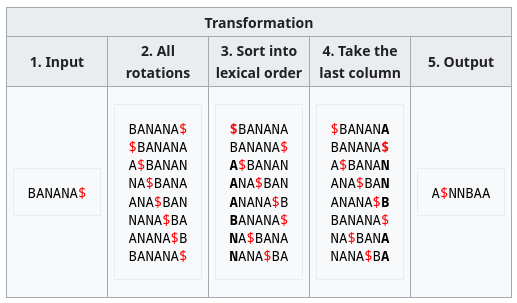
\includegraphics[scale=0.56]{images/bwt-example.png}
\end{frame}

\begin{frame}
	\frametitle{Prerequisites}
	\framesubtitle{Elastic Founder Graph: Block graph}
	\begin{definition}[Block Graph]
		We call \textbf{block graph} an undirected graph in which every biconnected
		component (i.e. a \textbf{block}) is a clique.
	\end{definition}
	\begin{center}
		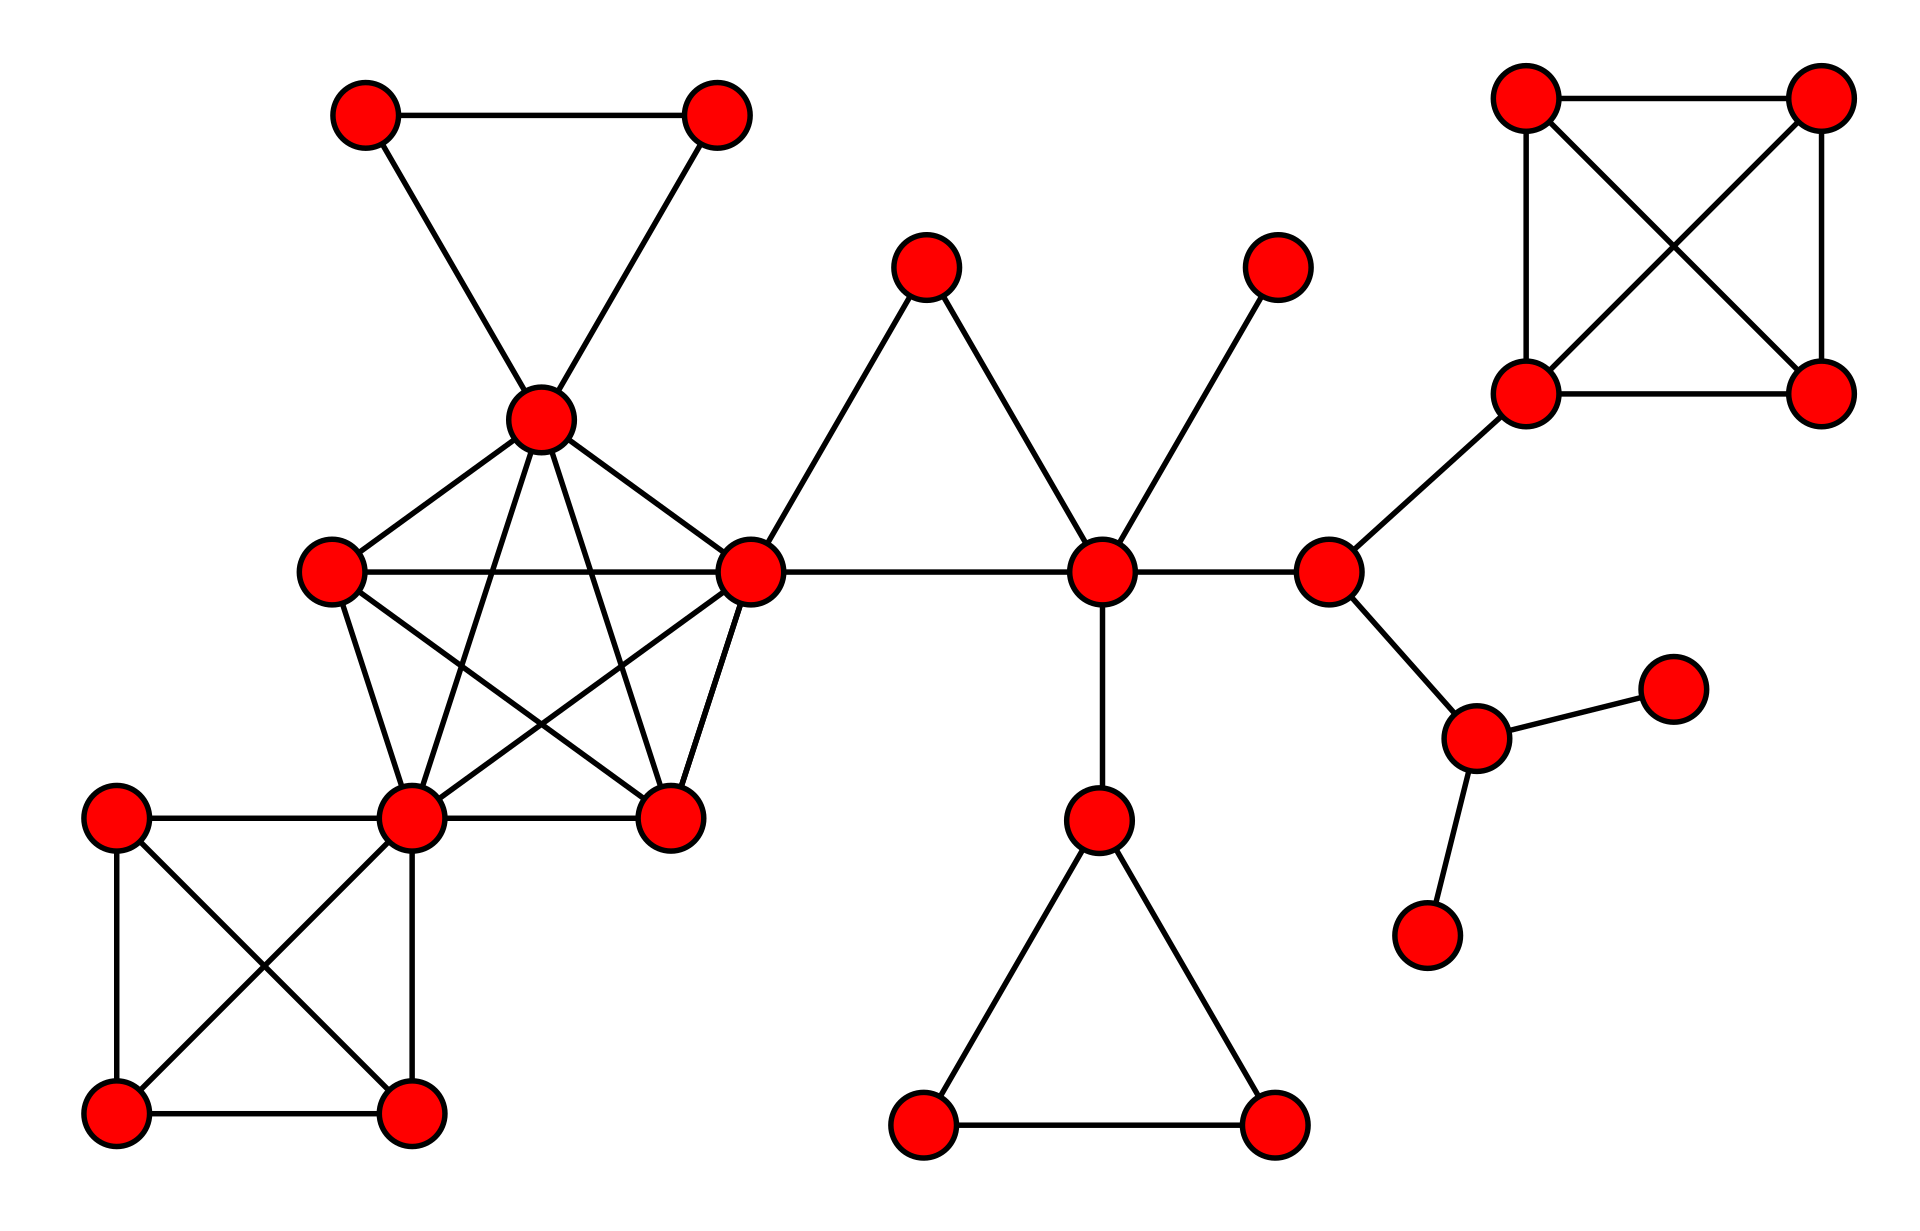
\includegraphics[scale=0.09]{images/block_graph.png}		
	\end{center}
\end{frame}

\begin{frame}
	\frametitle{Prerequisites}
	\framesubtitle{Elastic Founder Graph: definition}
	\begin{definition}[Elastic Founder Graph]
		Consider a block graph \(G = (V, E, l)\) with \(l: V \rightarrow \Sigma^+\). We call such a graph
		an \textbf{indexable Elastic Founder Graph} if the \textbf{semi-repeat-free} property holds: for each
		\(v\) in block \(V_i\), \(l(v)\) occurs in \(G\) only as prefix of paths starting with some
		\(w \in V_i\).
	\end{definition}
\end{frame}
\begin{frame}
	\frametitle{k-MEMs}
	\framesubtitle{k-MEMs: LEFTMAX, RIGHTMAX}
	Let \(Q \in \Sigma^+\) be a query string, \(\kappa\) be a threshold, \(lext(i, P, j)\) the left extension
	of the string \(P[i..j]\) and \(rext(i, P, j)\) the right extension.

	\onslide<2-3>\begin{definition}[LEFTMAX]
		A match \(([x..y], (i, P, j))\) of \(Q[x..y]\) in \(G\) satisfies the \(LEFTMAX\) property
		if and only if
		\[
			x = 1 \ \vee \ lext(i, P, j) = \emptyset \ \vee \ Q[x-1] \notin lext(i, P, j)
		\]
	\end{definition}

	\onslide<3>We can analogously define the RIGHTMAX property.
\end{frame}

\begin{frame}
	\frametitle{k-MEMs}
	\framesubtitle{k-MEMs: Definition}
	\begin{definition}[\(\kappa\)-MEM]
		A match \(([x..y], (i, P, j))\) of \(Q[x..y]\) in \(G\) is called a \(\kappa\)-MEM if it satisfies
		all the following conditions:
		\begin{enumerate}
			\item \(LEFTMAX \vee |lext(i, P, j)| \geq 2 \)
			\item \(RIGHTMAX \vee |rext(i, P, j)| \geq 2 \)
			\item \(y - x + 1 \geq \kappa\)
		\end{enumerate}
	\end{definition}
\end{frame}


\begin{frame}
	\frametitle{MEMs in Node Labels}
	\framesubtitle{Node MEMs: definition}
	\begin{definition}[Node MEM]
		A \(\kappa\)-MEM between a query string \(Q\) and the label \(l(v)\) of a vertex \(v \in V\)
		is called a node-MEM.
	\end{definition}

	\onslide<2-3>To give an algorithm to find node-MEMs we must consider the text
	\[
		T_{\text{nodes}} = \prod_{v \in V} 0 \times l(v).
	\]
	\onslide<3>We also need a data structure supporting the following operations over a bitvector \(B\):
	\begin{enumerate}
		\item \mintinline{python3}|r = rank(B, i)| in \(O(1)\) with \(r = \sum_{j=1}^{i} B[j]\),
		\item \mintinline{python3}|j = select(B, r)| in \(O(1)\) with \(j \leq i\) the position of
		the \(r\)-th 1 in \(B\).
	\end{enumerate}
\end{frame}

\begin{frame}
	\frametitle{MEMs in Node Labels}
	\framesubtitle{Algorithm to find k-node MEMs: prerequisites}
	We assume we have at our disposal the following procedures:
	\begin{enumerate}
		\item \mintinline{python3}|mems_using_bidirectional_bwts| which takes as input two
		bidirectional BWT indices on strings \(T, Q\) and a threshold \(\kappa\) and outputs
		\(Q'\) MEM strings with \(|Q'| \geq \kappa\) and for each string \(Q'\) four BWT intervals
		\(([i_T..j_T], [i'_T..j'_T], [i_Q..j_Q], [i'_Q..j'_Q])\) which represent the maximal
		matches of \(T\) and \(Q\) in \(O(|T| + |Q|)\) time;
		\onslide<2-3>\item \mintinline{python3}|mems_from_bidirectional_bwt| which takes as input four BWT
		intervals and outputs the corresponding MEM string \(Q'\) in \(O(|Q'|)\).
	\end{enumerate}
	\onslide<3> For both of these algorithms, one may refer to Algorithm 11.3 and Algorithm 11.4 from
	Genome-Scale Algorithm Design: Biological Sequence Analysis in the Era of High-Throughput Sequencing
	(Belazzougui et alia).
\end{frame}

\begin{frame}[fragile]
	\frametitle{MEMs in Node Labels}
	\framesubtitle{Algorithm to find k-node MEMs}
	We can now describe the algorithm to find node MEMs.
	\begin{enumerate}
		\onslide<2-6> \item We build a bitvector \(B\) to mark the location of 0s in \(T_{\text{nodes}}\)
		so that with the rank operation we can identify the corresponding node in G.
		\onslide<3-6>\item We call \mintinline{python3}|mems_using_bidirectional_bwts|
		using bidirectional BWT indices on strings \(T_{\text{nodes}}\) and \(Q\).
		\onslide<4-6>\item For each string \(Q'\) we get, we call
		\mintinline{python3}|mems_from_bidirectional_bwt| on its corresponding BWT intervals.
		\onslide<5-6>\item We use \(B\) to obtain the tuple \((i, P, j)\) in \(O(1)\) time.
	\end{enumerate}
	\onslide<6>The algorithm described above has complexity
	\(O(|T_{\text{nodes}}| + |Q| + N_{\kappa})\) with \(N_{\kappa}\) the number of output MEMs.
\end{frame}
\begin{frame}
	\frametitle{k-Node MEMs spanning exactly L nodes}
	\framesubtitle{Algorithm to find k-Node MEMs spanning exactly L nodes: prerequisites}
	\begin{enumerate}
		\item We call \(P^{L}_{G}\) a path of G spanning exactly \(L\) nodes.
		\onslide<2-3>\item We define two new symbols \(c\) and \(d\) not originally part of the alphabet \(\Sigma\)
		and the two operators:
		\begin{align*}
			left(u) &= \left\{
				\begin{array}{l}
					c \ \text{if} \ lext(u) = \{c\} \\
					\# \ \text{otherwise}
				\end{array}
			\right. && \\
			right(u) &= \left\{
				\begin{array}{l}
					d \ \text{if} \ rext(u) = \{d\} \\
					\# \ \text{otherwise}
				\end{array}
			\right.
		\end{align*}
		\onslide<3> \item We define the text
		\[
			T_L = 0 \times \prod_{u_1,..,u_L \in P^{L}_{G}}
			\Bigl(left(u_1) \times l(u_1) \times \dots \times l(u_L) \times right(u_L) \times 0\Bigr).
		\]
	\end{enumerate}
\end{frame}

\begin{frame}[fragile]
	\frametitle{k-Node MEMs spanning exactly L nodes}
	\framesubtitle{Algorithm to find k-Node MEMs spanning exactly L nodes}
	\begin{enumerate}
		\item  We modify the \mintinline{python3}|mems_from_bidirectional_bwt| so that it
		makes use of the symbols defined before we get the result using the
		algorithm we defined for \(\kappa\)-node MEMs.
		\onslide<2-4>\item The complexity we get is \(O(|T_L| + |Q| + M_{\kappa, L})\) with \(M_{\kappa, L}\)
		the number of output MEMs.
		\onslide<3-4>\item Let \(d\) be the maximum in-degree (or out-degree) of a node, \(n\) the total label length
		of \(G\). Now we can reformulate the time complexity.
		
		\onslide<4>\item \(|T_L|\) is the concatenation of paths of \(G\) of length \(L\):
		for a node \(v\) the number of paths containing \(l(v)\)
		is at most \(L \times d^{L-1}\). The complexity can be rewritten as
		\(O(|Q| + M_{\kappa, L } + n \times L \times d^{L-1})\) which is exponential on \(L\).
	\end{enumerate}
\end{frame}
\begin{frame}
	\frametitle{MEMs in EFGs}
	\framesubtitle{k-Node MEMs in EFGs: Remark}
	\begin{remark}
		Given an indexable EFG \(G = (V, E, l)\), for each \((v, w) \in E\)
		string \(l(v)l(w)\) occurs only as prefix of paths starting with \(v\).
	\end{remark}
	\onslide<2-3>Rephrasing what is written above, all occurrences of some string \(S\) in \(G\) spanning at
	least four nodes can be decomposed as \(\alpha l(u_2 ) \dots l(u_{L-1})\beta\) such that:
	\begin{enumerate}
		\item \(u_2 \dots u_{L-1}\) is a path in \(G\) and \(u_2, \dots , u_{L-1}\)
		are unequivocally identified;
		\item \(\alpha = l(u_1)[i..||u_1||]\) with \(1 \leq i \leq ||u_1||\) for some \((u_1, u_2 ) \in E\);
		\item \(\beta = l(u_L)\) for some \((u_{L-1} , u_L ) \in E\)
		or \(\beta = l(uL )(l(uL+1 )[1..j])\) with \(1 \leq j \leq ||u_{L+1}||\)
		for some \((u_{L-1} , u_L )\), \((u_L , u_{L+1} ) \in E\).
	\end{enumerate}
	\onslide<3>Note that \(\alpha, \beta \neq \epsilon\) and \(\beta\) has as prefix a full node label,
	\(\alpha\) might spell any suffix of a node label.
\end{frame}

\begin{frame}
	\frametitle{MEMs in EFGs}
	\framesubtitle{k-Node MEMs in EFGs spanning more than 3 nodes: preprocessing}
	First, we take the text
	\(
		T'_3 = \prod_{(u, v), (v, w) \in E} \bigl(l(u)l(v)l(w) \times 0\bigr).
	\)
	\begin{enumerate}
		\item \onslide<2-5> We mark all implicit or explicit nodes \(\bar{p}\) such that the
		corresponding root-to-\(\bar{p}\) path spells
		\(l(u)l(v)\) for some \((u, v) \in E\), so that we can query in constant time if $\bar{p}$
		is such a node.
		\item \onslide<3-5> We compute pointers from each node $\bar{p}$ to an arbitrarily chosen
		leaf in the subtree rooted at $\bar{p}$;
		\item \onslide<4-5>for each node \(v \in V\) of the indexable EFG we build trie $T_v$ for the
		set of strings ${\bar{l(u)}: (u, v) \in E}$;
		\item \onslide<5> for each leaf, we store the corresponding path \(uvw\) and the starting
		position of the suffix inside \(l(u)l(v)l(w)\).
	\end{enumerate}
\end{frame}

\begin{frame}
	\frametitle{MEMs in EFGs}
	\framesubtitle{k-Node MEMs in EFGs spanning more than 3 nodes: processing}
	Let \(\bar{p}\) be the suffix tree node of \(T'_3\) reached from the root by spelling
	\(Q[1..y]\) in the suffix tree until we cannot continue with \(Q[y+1]\):
	\begin{enumerate}
		\onslide<2-4>\item If we cannot continue with a \(0\), \(Q[1..y]\) spans no more than 3 nodes, so we can discard
		it. We can now consider matching \(Q[2..y]\) in \(G\) taking the suffix link of \(\bar{p}\).
		\onslide<3-4>\item If we can continue with a \(0\) and the occurrences of \(Q[1..y]\) span no more
		than 2 nodes, we proceed as in the previous step.
		\onslide<4>\item In this case, \(Q[1..y] = \alpha l(u_2)l(u_3)\) for exactly one \(u_2 \in V\),
		with \((u_2, u_3) \in E\), we follow the suffix link walk from \(\bar{p}\) until we find the marked
		node \(\bar{q}\) corresponding to \(l(u_2)l(u_3)\): from \(\bar{q}\) we try to
		match \(Q[y + 1..]\) until failure, matching \(Q[y + 1..y']\) and reaching node \(\bar{r}\).
	\end{enumerate}
\end{frame}

\begin{frame}
	\frametitle{MEMs in EFGs}
	\framesubtitle{Algorithm complexity}
	\begin{theorem}[Algorithm complexity]
		Let alphabet \(\Sigma\) be of constant size, and let G = \((V, E, l)\) be an indexable
		Elastic Founder Graph of height \(H\), that is, the maximum number of nodes in a block of
		\(G\) is \(H\).
		The algorithm to find \(\kappa\)-node-MEMs spanning \(L>3\) nodes has time complexity
		\(O(nH^2 + |Q| + M_\kappa)\) with \(n = \sum_{v \in V}|v|\) and \(M_\kappa\) the number
		of output MEMs.
	\end{theorem}
	\onslide<2>\begin{proof}
		It derives from the complexity of the algorithm to find \(\kappa\)-node MEMs spanning exactly
		\(L\) nodes given before.
	\end{proof}
\end{frame}
\begin{frame}
	\frametitle{Corollaries}
	\begin{corollary}
		The results we have given for \(\kappa\)-node MEMs, \(\kappa\)-node MEMs spanning
		exactly \(L\) nodes and EFGs hold when \(Q[1..m]\) is replaced by a set of
		queries of total length \(m\).
	\end{corollary}
	\onslide<2>\begin{corollary}
		The algorithms we have given before (including the corollary above) can be modified
		to report only MEMs that occur in text \(T\) formed by concatenating the rows (ignoring
		gaps and adding separator symbols) of the input MSA of the indexable EFG.
	\end{corollary}
	This can be done in additional \(O(|T | + r \log r)\) time and \(O(r \log n)\) bits of space,
	and with multiplicative factor \(O(\log \log n)\) added to the running times
	of the respective algorithms, where \(r\) is the number of equal-letter runs in the BWT of \(T\).
\end{frame}

\begin{frame}
	\frametitle{Experimental results}
	\framesubtitle{Number of MEMs with different indices and varying number of covid19 strains}
	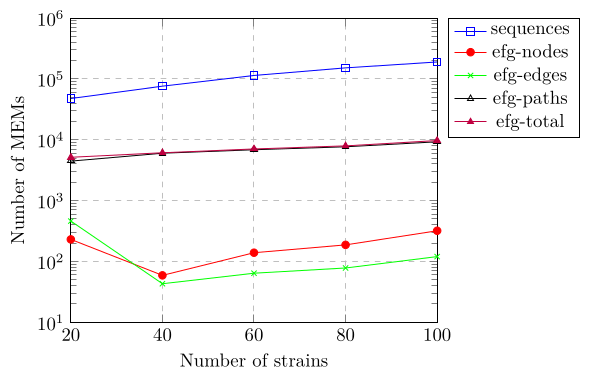
\includegraphics[scale=0.5]{images/number-of-mems.png}
\end{frame}

\begin{frame}
	\frametitle{Experimental results}
	\framesubtitle{Number of BWT runs with different indexes and varying number of covid19 strains}
	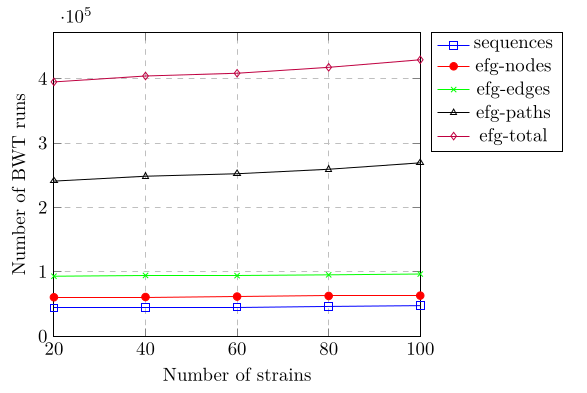
\includegraphics[scale=0.5]{images/number-of-bwt-runs.png}
\end{frame}
\end{document}